\appendix
\section{Sensitivity curves}\label{app:a}
The plots in this section show all of the detectors and sources described in the main text. Clearer, interactive versions of these plots, allowing for removal of any of the curves, may be created and downloaded on-line, \url{http://rhcole.com/apps/GWplotter}. The detector noise curves all have their resonance spikes removed for clarity. 

\begin{figure}
 \centering
 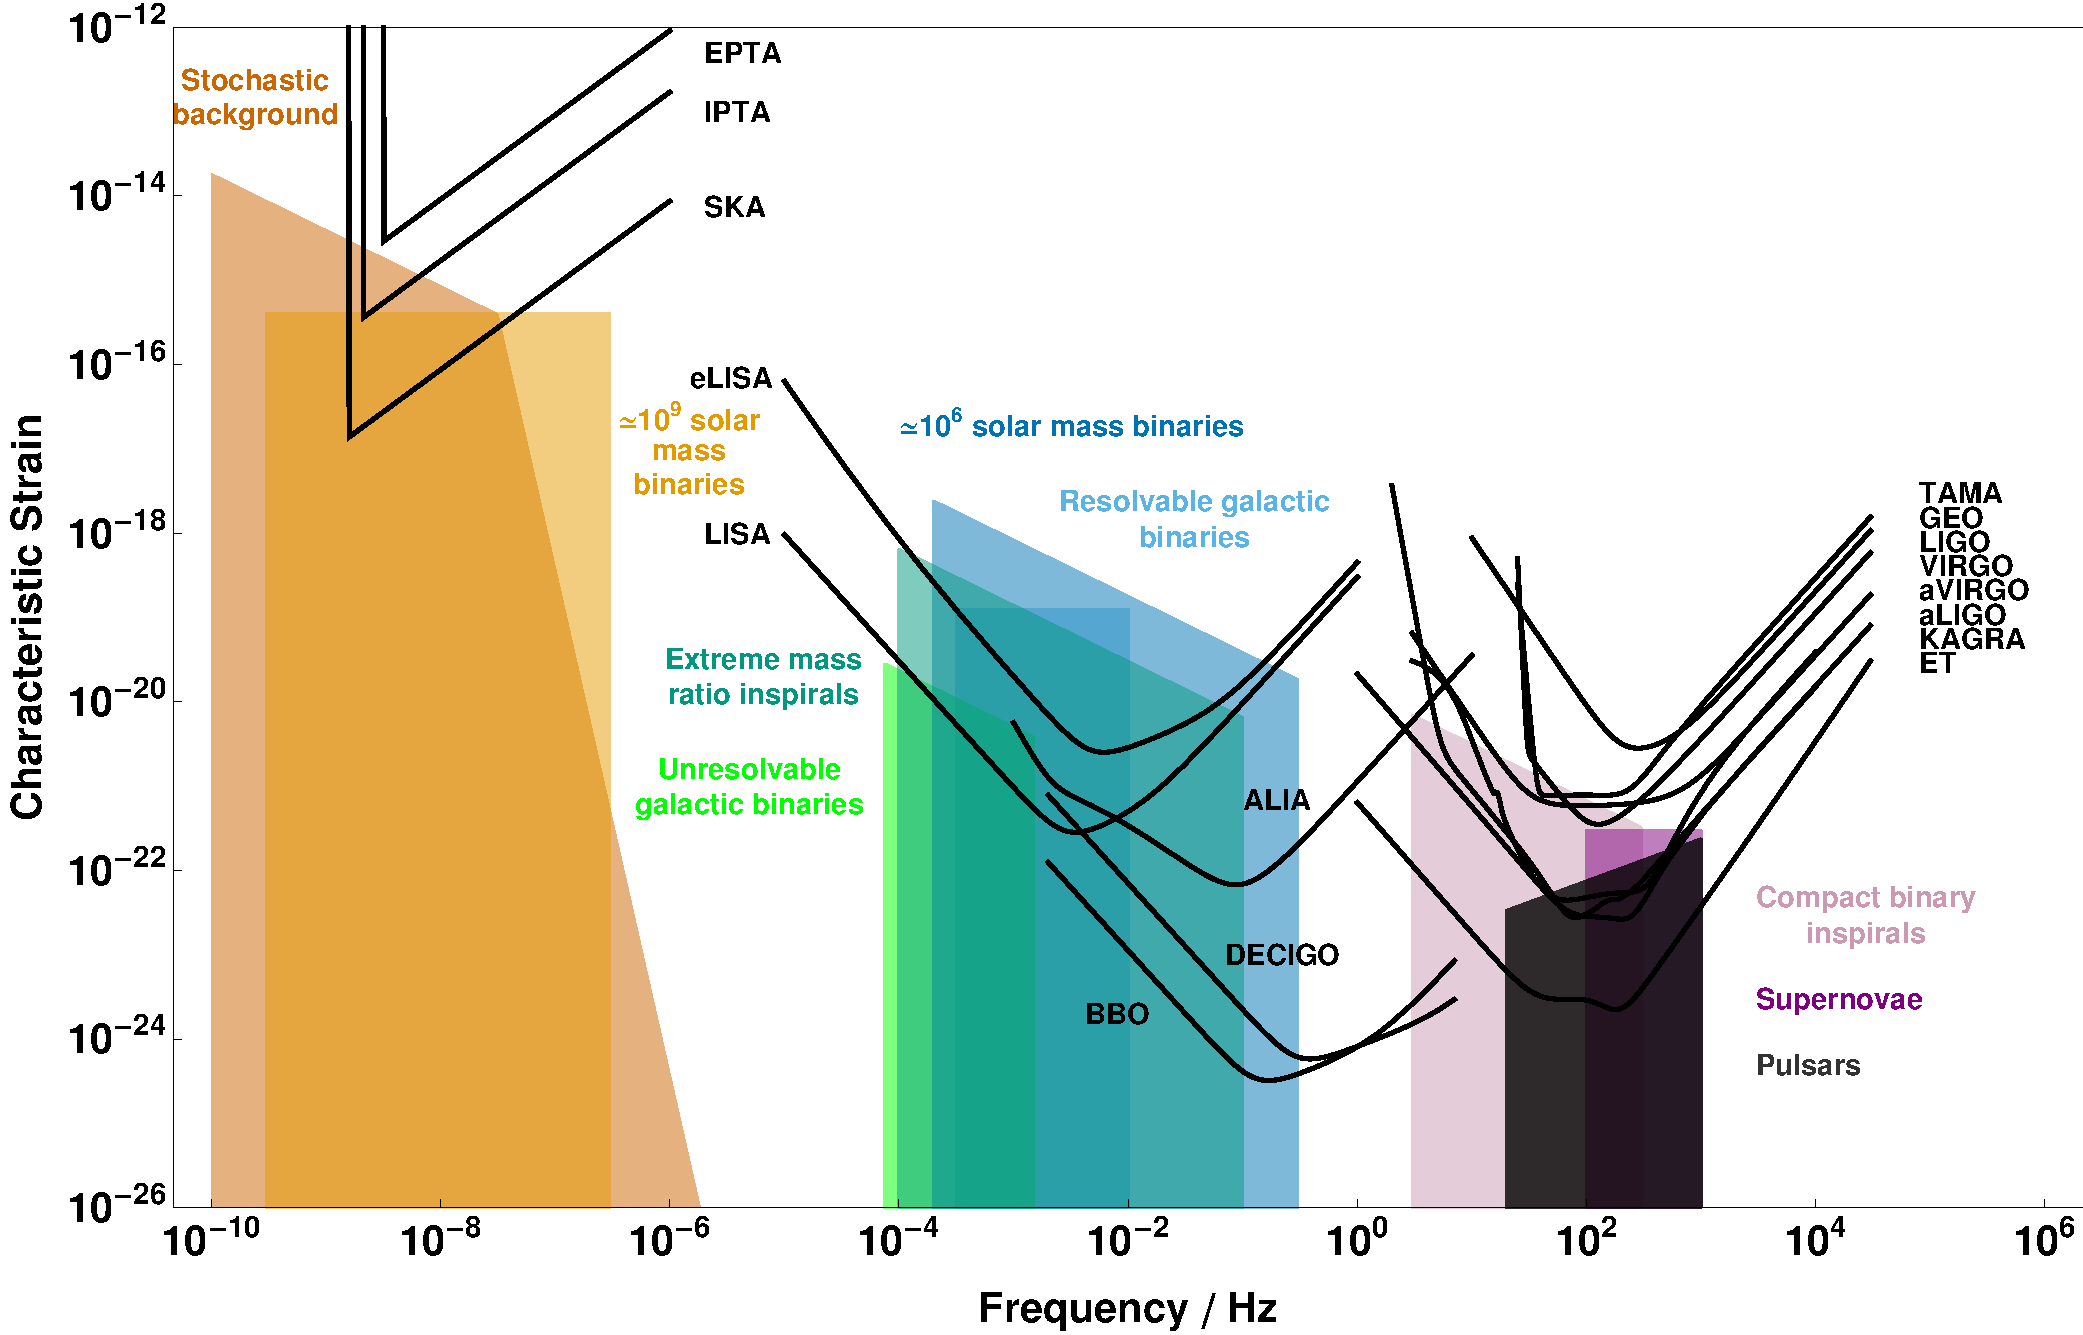
\includegraphics[trim=0cm 0cm 0cm 0cm, width=0.8\textwidth]{figure1.pdf}
 \caption{A plot of characteristic strain against frequency for a variety of detectors and sources.}
 \label{fig:hc}
\end{figure}

\begin{figure}
 \centering
 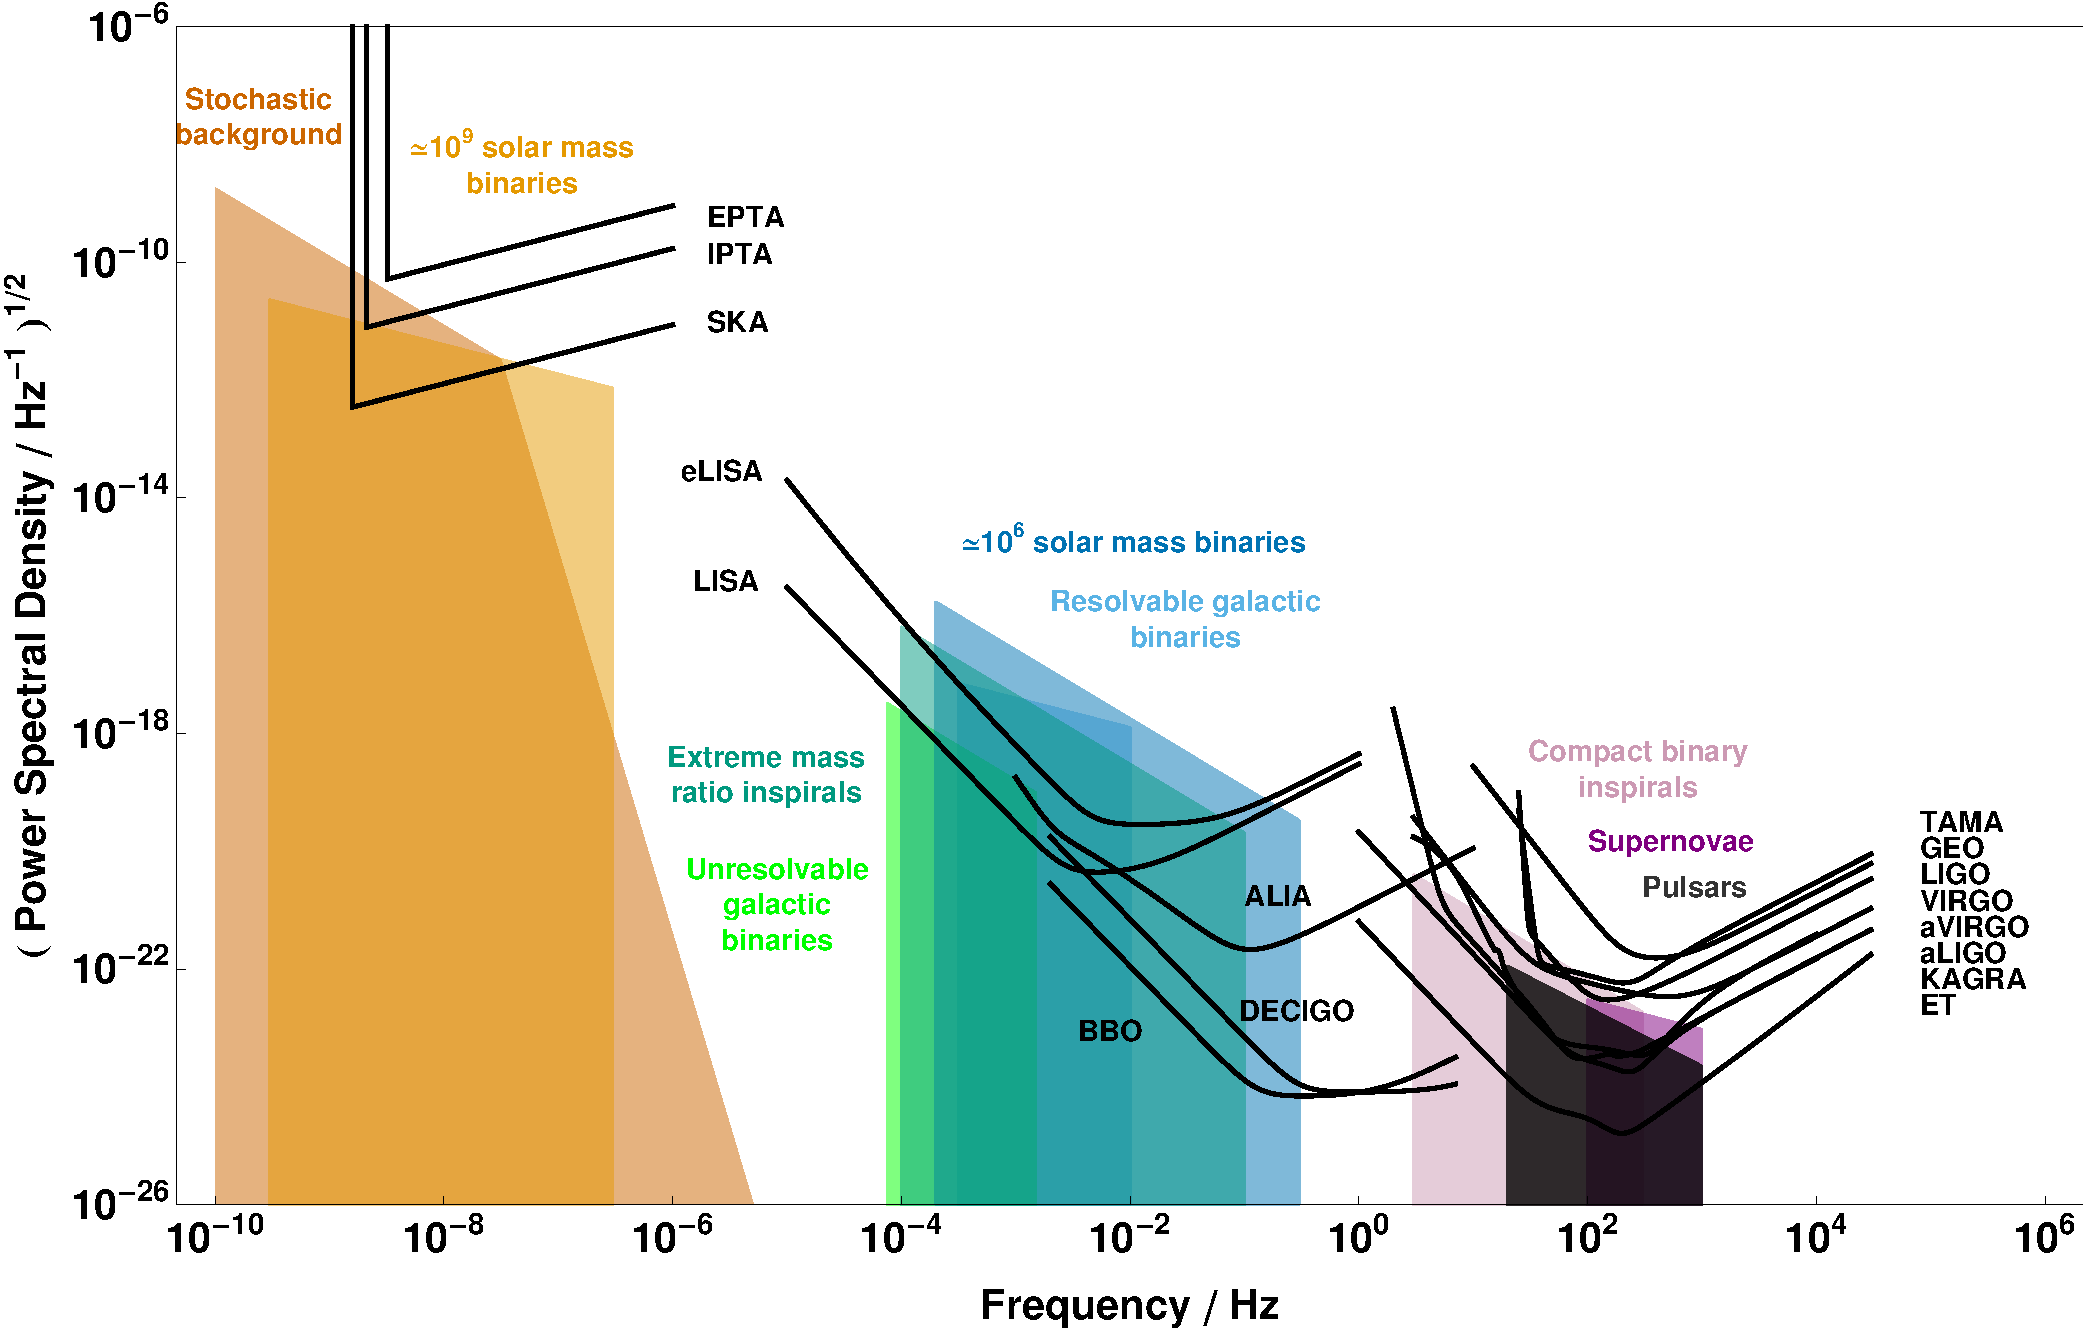
\includegraphics[trim=0cm 0cm 0cm 0cm, width=0.8\textwidth]{figure2.pdf}
 \caption{A plot of the square root of power spectral density against frequency for a variety of detectors and sources.}
 \label{fig:S}
\end{figure}

\begin{figure}
 \centering
 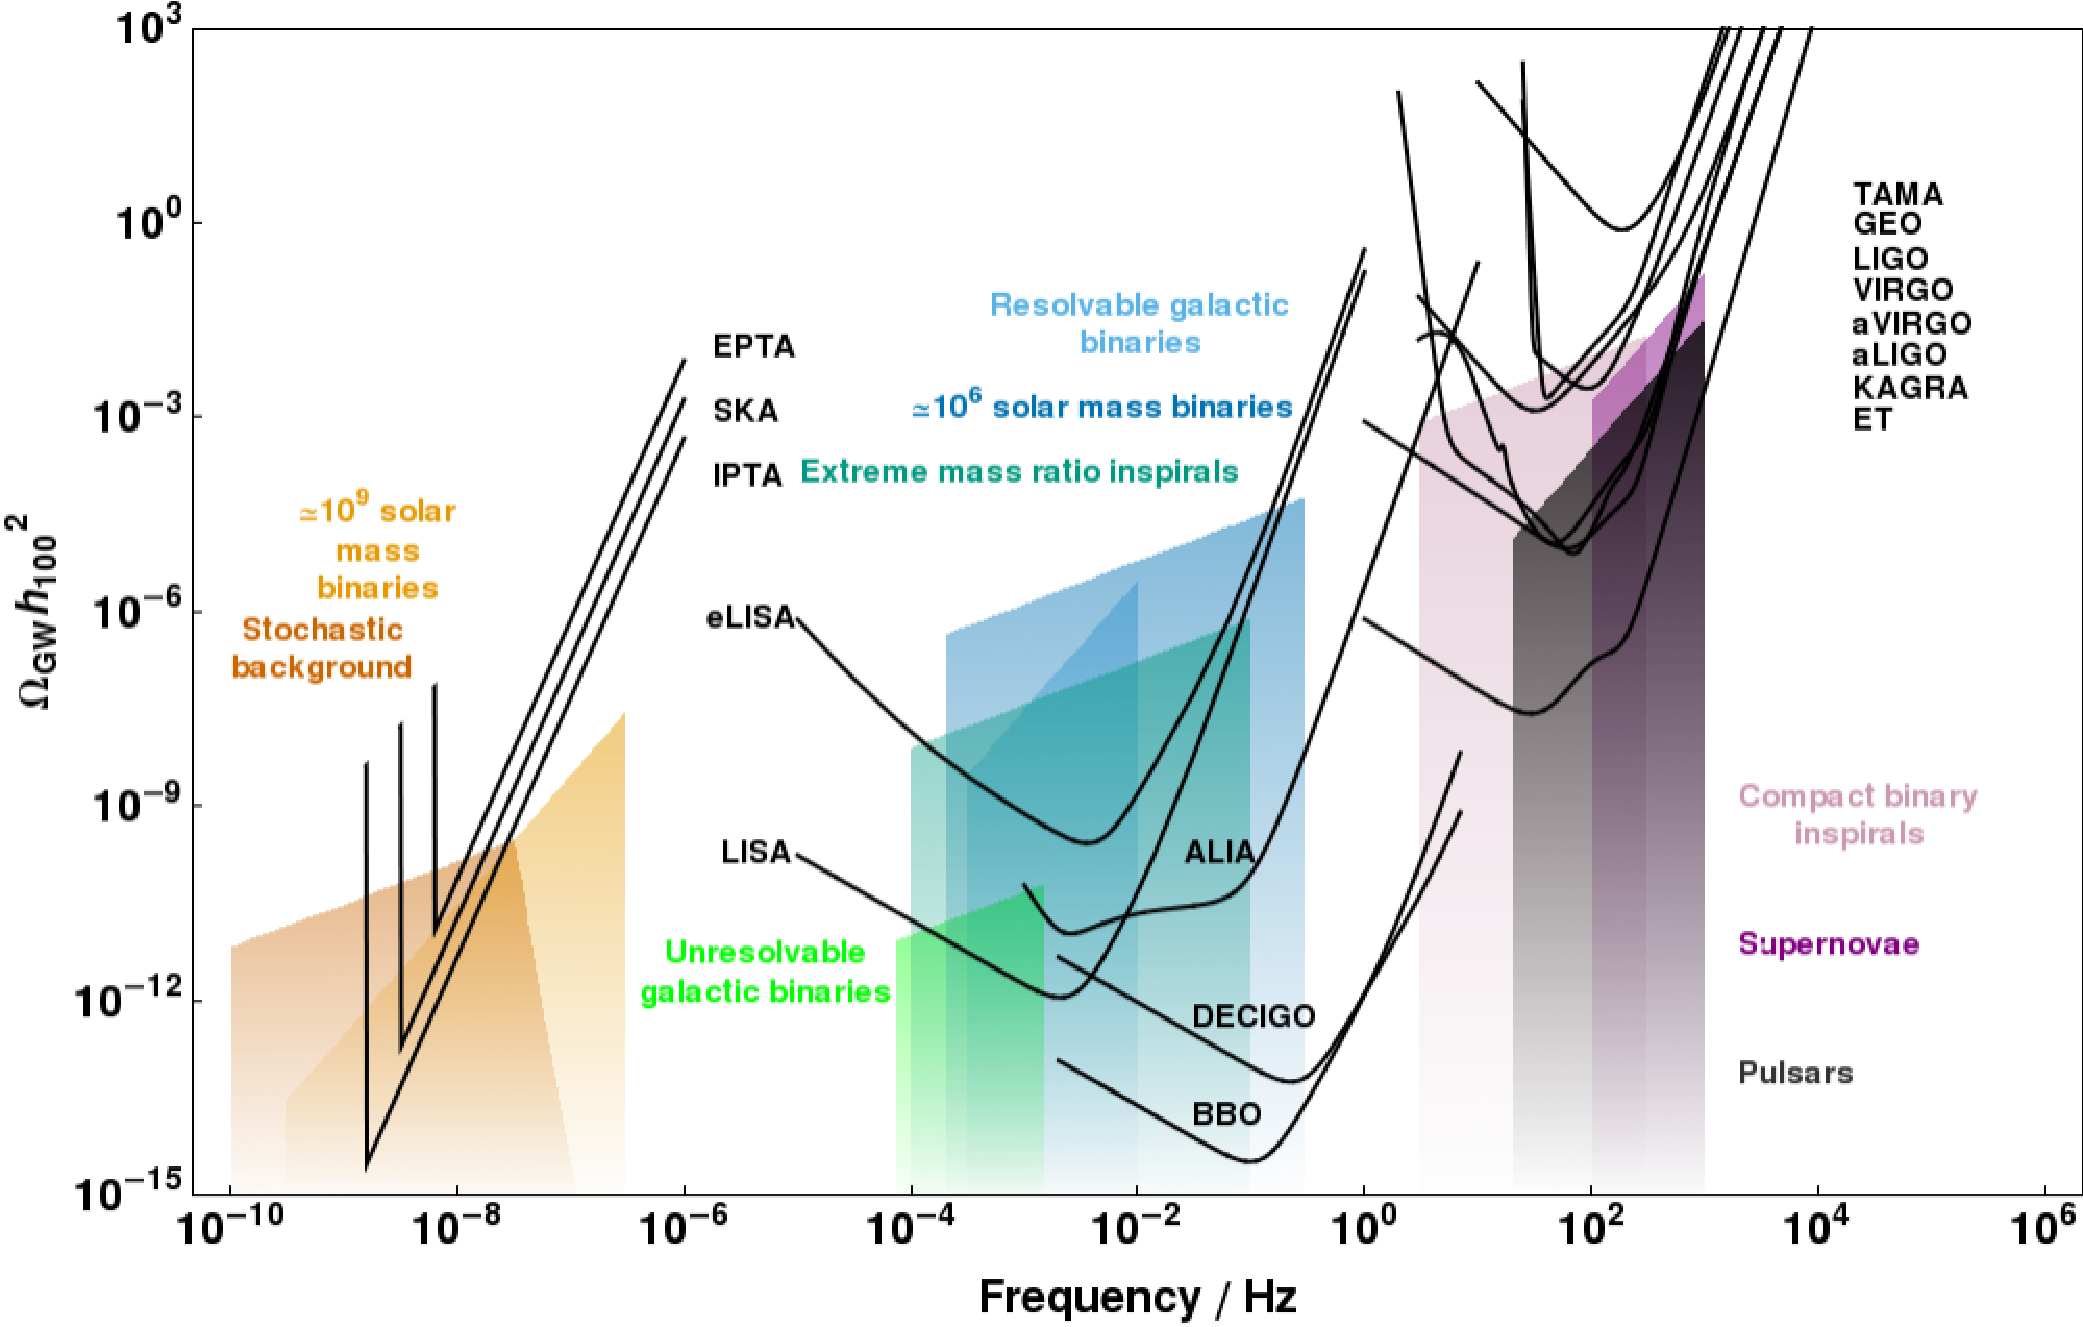
\includegraphics[trim=0cm 0cm 0cm 0cm, width=0.8\textwidth]{figure3.pdf}
 \caption{A plot of the dimensionless energy density in GWs against frequency for a variety of detectors and sources.}
 \label{fig:omega}
\end{figure}


